\documentclass[10pt,a4paper]{article}
\usepackage[margin=16mm]{geometry}
\usepackage{booktabs,graphicx,amsmath,xcolor,hyperref}
\hypersetup{colorlinks=true,urlcolor=blue,linkcolor=blue,pdftitle={Results Checkpoint: PPE Safety Equipment Detection},pdfauthor={P14 project team}}
\graphicspath{{../../reports/results_checkpoint/figures/}}
\setlength{\parindent}{0pt}
\setlength{\parskip}{4pt}
\setlength{\tabcolsep}{5pt}
\renewcommand{\arraystretch}{1.08}
\newcommand{\APgain}{0.0028}
\newcommand{\Fgain}{0.0288}
\newcommand{\LatencyRatio}{1.59}

\begin{document}
\begin{center}
{\Large\bfseries Results Checkpoint: PPE Safety Equipment Detection}\\[3pt]
P14 --- Computer Vision 2026 --- 2 November 2026
\end{center}
\section*{1. Completed experimental evaluation}
We compare COCO-pretrained YOLO11n and YOLO11s on all 11 Construction-PPE classes. The frozen split contains 1,265 training, 73 validation and \textbf{78 test images (924 boxes)}. Both models were fine-tuned for 50 epochs, batch 16, 640-pixel inputs, SGD learning rate 0.01, momentum 0.937, weight decay 0.0005, three warm-up epochs and cosine decay. Training uses flips and mild scale/translation/HSV augmentation, without mosaic, mixup or copy-paste. We report all seeds 42, 43 and 44, selecting each checkpoint by validation mAP50:95.

Stage 4 selected confidence \textbf{0.20 for YOLO11n and 0.30 for YOLO11s} by mean validation macro-F1. These values and the six checkpoint hashes were frozen before test inference. There is no test threshold sweep or test-based seed selection. Both models use square letterboxing to $640\times640$, FP32, class-aware NMS IoU 0.70 and at most 300 detections. AP uses confidence 0.001, library multi-label expansion and IoU thresholds 0.50:0.05:0.95. Fixed-threshold metrics use standard single-label predictions and greedy, same-class, one-to-one matching in descending IoU order at IoU $\geq0.50$. Macro-F1 is the mean of the 11 class F1 scores, $F1_c=2TP_c/(2TP_c+FP_c+FN_c)$; macro P/R average class P/R. All test classes have ground truth.
\begin{center}\small\begin{tabular}{lrr}
\toprule
Test metric & YOLO11n & YOLO11s \\
\midrule
mAP@0.50:0.95 & 0.1874 $\pm$ 0.0037 & 0.1902 $\pm$ 0.0067 \\
mAP@0.50 & 0.4413 $\pm$ 0.0150 & 0.4505 $\pm$ 0.0203 \\
Macro precision & 0.4731 $\pm$ 0.0547 & 0.5512 $\pm$ 0.0307 \\
Macro recall & 0.4632 $\pm$ 0.0061 & 0.4525 $\pm$ 0.0164 \\
Macro-F1 & 0.4547 $\pm$ 0.0238 & 0.4835 $\pm$ 0.0218 \\
Macro-F1 (reference confidence 0.25) & 0.4593 $\pm$ 0.0211 & 0.4791 $\pm$ 0.0218 \\
\bottomrule
\end{tabular}
\end{center}
All values are \textbf{mean $\pm$ sample SD across three seeds}, not confidence intervals. P/R/F1 use each model's frozen threshold; AP is a ranked-prediction metric. YOLO11s gains \APgain{} absolute mAP50:95 and \Fgain{} macro-F1, with higher precision but slightly lower recall. The AP gain is small relative to seed variation and does not establish statistical significance. YOLO11n's reference F1 at 0.25 exceeds its selected-threshold test F1; we retain 0.20 to respect validation-only selection.
\begin{center}\small\begin{tabular}{lrrrrrr}
\toprule
Model & Seed & mAP50:95 & mAP50 & Macro P & Macro R & Macro-F1 \\
\midrule
yolo11n & 42 & 0.1905 & 0.4547 & 0.5056 & 0.4625 & 0.4739 \\
yolo11n & 43 & 0.1833 & 0.4251 & 0.4100 & 0.4574 & 0.4280 \\
yolo11n & 44 & 0.1885 & 0.4441 & 0.5039 & 0.4695 & 0.4621 \\
yolo11s & 42 & 0.1825 & 0.4279 & 0.5275 & 0.4336 & 0.4594 \\
yolo11s & 43 & 0.1933 & 0.4565 & 0.5403 & 0.4620 & 0.4890 \\
yolo11s & 44 & 0.1947 & 0.4672 & 0.5859 & 0.4620 & 0.5020 \\
\bottomrule
\end{tabular}
\end{center}
\section*{2. Runtime and computational cost}
\begin{center}\small\begin{tabular}{lrrrrr}
\toprule
Model & Params (M) & Weights (MB) & CPU ms & IQR (ms) & Train min/seed \\
\midrule
yolo11n & 2.61 & 5.51 & 50.21 & 46.26--53.38 & 50.7 $\pm$ 0.9 \\
yolo11s & 9.43 & 19.18 & 79.80 & 68.08--85.78 & 88.9 $\pm$ 0.1 \\
\bottomrule
\end{tabular}
\end{center}
\textbf{New controlled CPU benchmark:} Apple M2 Max (Ultralytics CPU identification), four PyTorch threads, batch one, FP32, seed 42, confidence 0.25; 20 warm-up and 100 timed calls per model on the same ordered, in-memory test images. Median and interquartile range (IQR) include preprocessing, forward inference, NMS and predict-call overhead; disk reading, loading weights and plotting are excluded. YOLO11s costs \LatencyRatio{} times the median latency. Parameter counts are from the unfused checkpoints; MB means $10^6$ bytes.

Training wall times used Apple M4/MPS for YOLO11n and M2 Max/MPS for YOLO11s (three concurrent jobs, CPU loss/NMS workaround). They are \textbf{not a controlled training-speed comparison}. Historical Stage 4 MPS medians (7.58/10.03 ms) are separate from these CPU results. Test software: Python 3.14.7, PyTorch 2.14.1, Ultralytics 8.4.175, macOS 15.7.2 arm64.
\newpage
\section*{3. Class performance and difficult subsets}
\begin{center}\small\begin{tabular}{lrrrrrr}
\toprule
Class & Train & Test & AP50 (n) & AP50 (s) & Recall (n) & Recall (s) \\
\midrule
helmet & 1454 & 161 & 0.903 $\pm$ 0.005 & 0.904 $\pm$ 0.008 & 0.882 $\pm$ 0.006 & 0.878 $\pm$ 0.013 \\
gloves & 1351 & 57 & 0.322 $\pm$ 0.018 & 0.351 $\pm$ 0.023 & 0.357 $\pm$ 0.027 & 0.322 $\pm$ 0.037 \\
vest & 1376 & 150 & 0.830 $\pm$ 0.015 & 0.812 $\pm$ 0.027 & 0.833 $\pm$ 0.013 & 0.813 $\pm$ 0.040 \\
boots & 1413 & 144 & 0.339 $\pm$ 0.023 & 0.352 $\pm$ 0.014 & 0.412 $\pm$ 0.083 & 0.377 $\pm$ 0.021 \\
goggles & 501 & 9 & 0.106 $\pm$ 0.065 & 0.202 $\pm$ 0.115 & 0.037 $\pm$ 0.064 & 0.111 $\pm$ 0.111 \\
none & 677 & 51 & 0.558 $\pm$ 0.085 & 0.558 $\pm$ 0.009 & 0.673 $\pm$ 0.011 & 0.647 $\pm$ 0.020 \\
Person & 1884 & 198 & 0.768 $\pm$ 0.032 & 0.782 $\pm$ 0.017 & 0.790 $\pm$ 0.026 & 0.783 $\pm$ 0.013 \\
no\_helmet & 400 & 40 & 0.377 $\pm$ 0.051 & 0.312 $\pm$ 0.044 & 0.442 $\pm$ 0.095 & 0.375 $\pm$ 0.025 \\
no\_goggle & 337 & 33 & 0.382 $\pm$ 0.086 & 0.486 $\pm$ 0.080 & 0.424 $\pm$ 0.061 & 0.465 $\pm$ 0.063 \\
no\_gloves & 442 & 58 & 0.157 $\pm$ 0.040 & 0.153 $\pm$ 0.006 & 0.172 $\pm$ 0.034 & 0.178 $\pm$ 0.010 \\
no\_boots & 88 & 23 & 0.111 $\pm$ 0.011 & 0.043 $\pm$ 0.019 & 0.072 $\pm$ 0.066 & 0.029 $\pm$ 0.025 \\
\bottomrule
\end{tabular}
\end{center}
Counts are ground-truth boxes; AP50 and recall are mean $\pm$ SD across seeds. Full AP50:95, precision, F1 and TP/FP/FN counts are exported per class and seed. Helmet, vest and Person are strongest. Goggles (only nine test boxes) and missing-equipment classes remain difficult; \texttt{no\_boots} AP50 is lower for YOLO11s. Thus increasing model size does not improve every class. Class imbalance is relevant, but object scale, ambiguous source boxes and domain diversity also affect performance; these data do not isolate a causal imbalance effect.
\begin{center}\small\begin{tabular}{lrrr}
\toprule
Object subset & Count & Recall (n) & Recall (s) \\
\midrule
size: small & 98 & 0.354 $\pm$ 0.026 & 0.310 $\pm$ 0.012 \\
size: medium & 469 & 0.548 $\pm$ 0.013 & 0.527 $\pm$ 0.018 \\
size: large & 357 & 0.810 $\pm$ 0.018 & 0.810 $\pm$ 0.010 \\
visibility: clear & 259 & 0.835 $\pm$ 0.010 & 0.829 $\pm$ 0.022 \\
visibility: occluded & 72 & 0.676 $\pm$ 0.021 & 0.676 $\pm$ 0.069 \\
visibility: uncertain & 190 & 0.432 $\pm$ 0.045 & 0.388 $\pm$ 0.008 \\
truncated: yes & 24 & 0.819 $\pm$ 0.024 & 0.833 $\pm$ 0.042 \\
truncated: no & 309 & 0.796 $\pm$ 0.006 & 0.790 $\pm$ 0.034 \\
truncated: uncertain & 188 & 0.433 $\pm$ 0.048 & 0.388 $\pm$ 0.011 \\
\bottomrule
\end{tabular}
\end{center}
\textbf{Size:} all 924 objects are partitioned using box area after aspect-preserving resize to 640 pixels: small $A<32^2$, medium $32^2\leq A<96^2$, large $A\geq96^2$. Matching is done on the full image first; subgroup recall then counts matched targets, so a prediction cannot be reused across groups. This is object-weighted recall, not macro recall. Class-by-size results appear in Section 5. Both models miss most small objects, and YOLO11s has lower small-object recall at its frozen operating point. These thresholds differ, so the comparison combines model and deployment-threshold effects.

\textbf{Visibility and truncation:} these rows cover only the five PPE classes (521 objects). The primary visibility comparison uses 259 clear and 72 occluded objects; 190 uncertain objects are excluded from that comparison and shown separately for transparency. Occluded recall is 0.676 for both models, versus approximately 0.83 for clear PPE. These are observational associations, not an isolated occlusion effect. Size distributions differ:
\begin{center}\small\begin{tabular}{lrrr}
\toprule
PPE visibility & Small & Medium & Large \\
\midrule
clear & 13 & 175 & 71 \\
occluded & 1 & 33 & 38 \\
uncertain & 49 & 135 & 6 \\
\bottomrule
\end{tabular}
\end{center}
The groups also differ in class composition: 58 of 72 occluded objects are vests; occluded goggles have no support. The truncation rows are a separate partition (24 yes, 309 no, 188 uncertain); higher recall for the small truncated group does not imply truncation helps detection. \textbf{Review limitation:} visibility/truncation labels come from one assistant visual review before predictions, not two independent human reviewers; the planned Member 4 review has not occurred. Class-specific counts and recalls, including sparse groups, are provided in the CSV outputs.
\newpage
\section*{Visual comparison of test performance}
The plots summarize the same measurements as Section 3; tables retain the exact values. Error bars show \textbf{sample standard deviation across seeds 42, 43 and 44}, not confidence intervals. Counts $n$ refer to ground-truth objects in the fixed test split.
\begin{center}
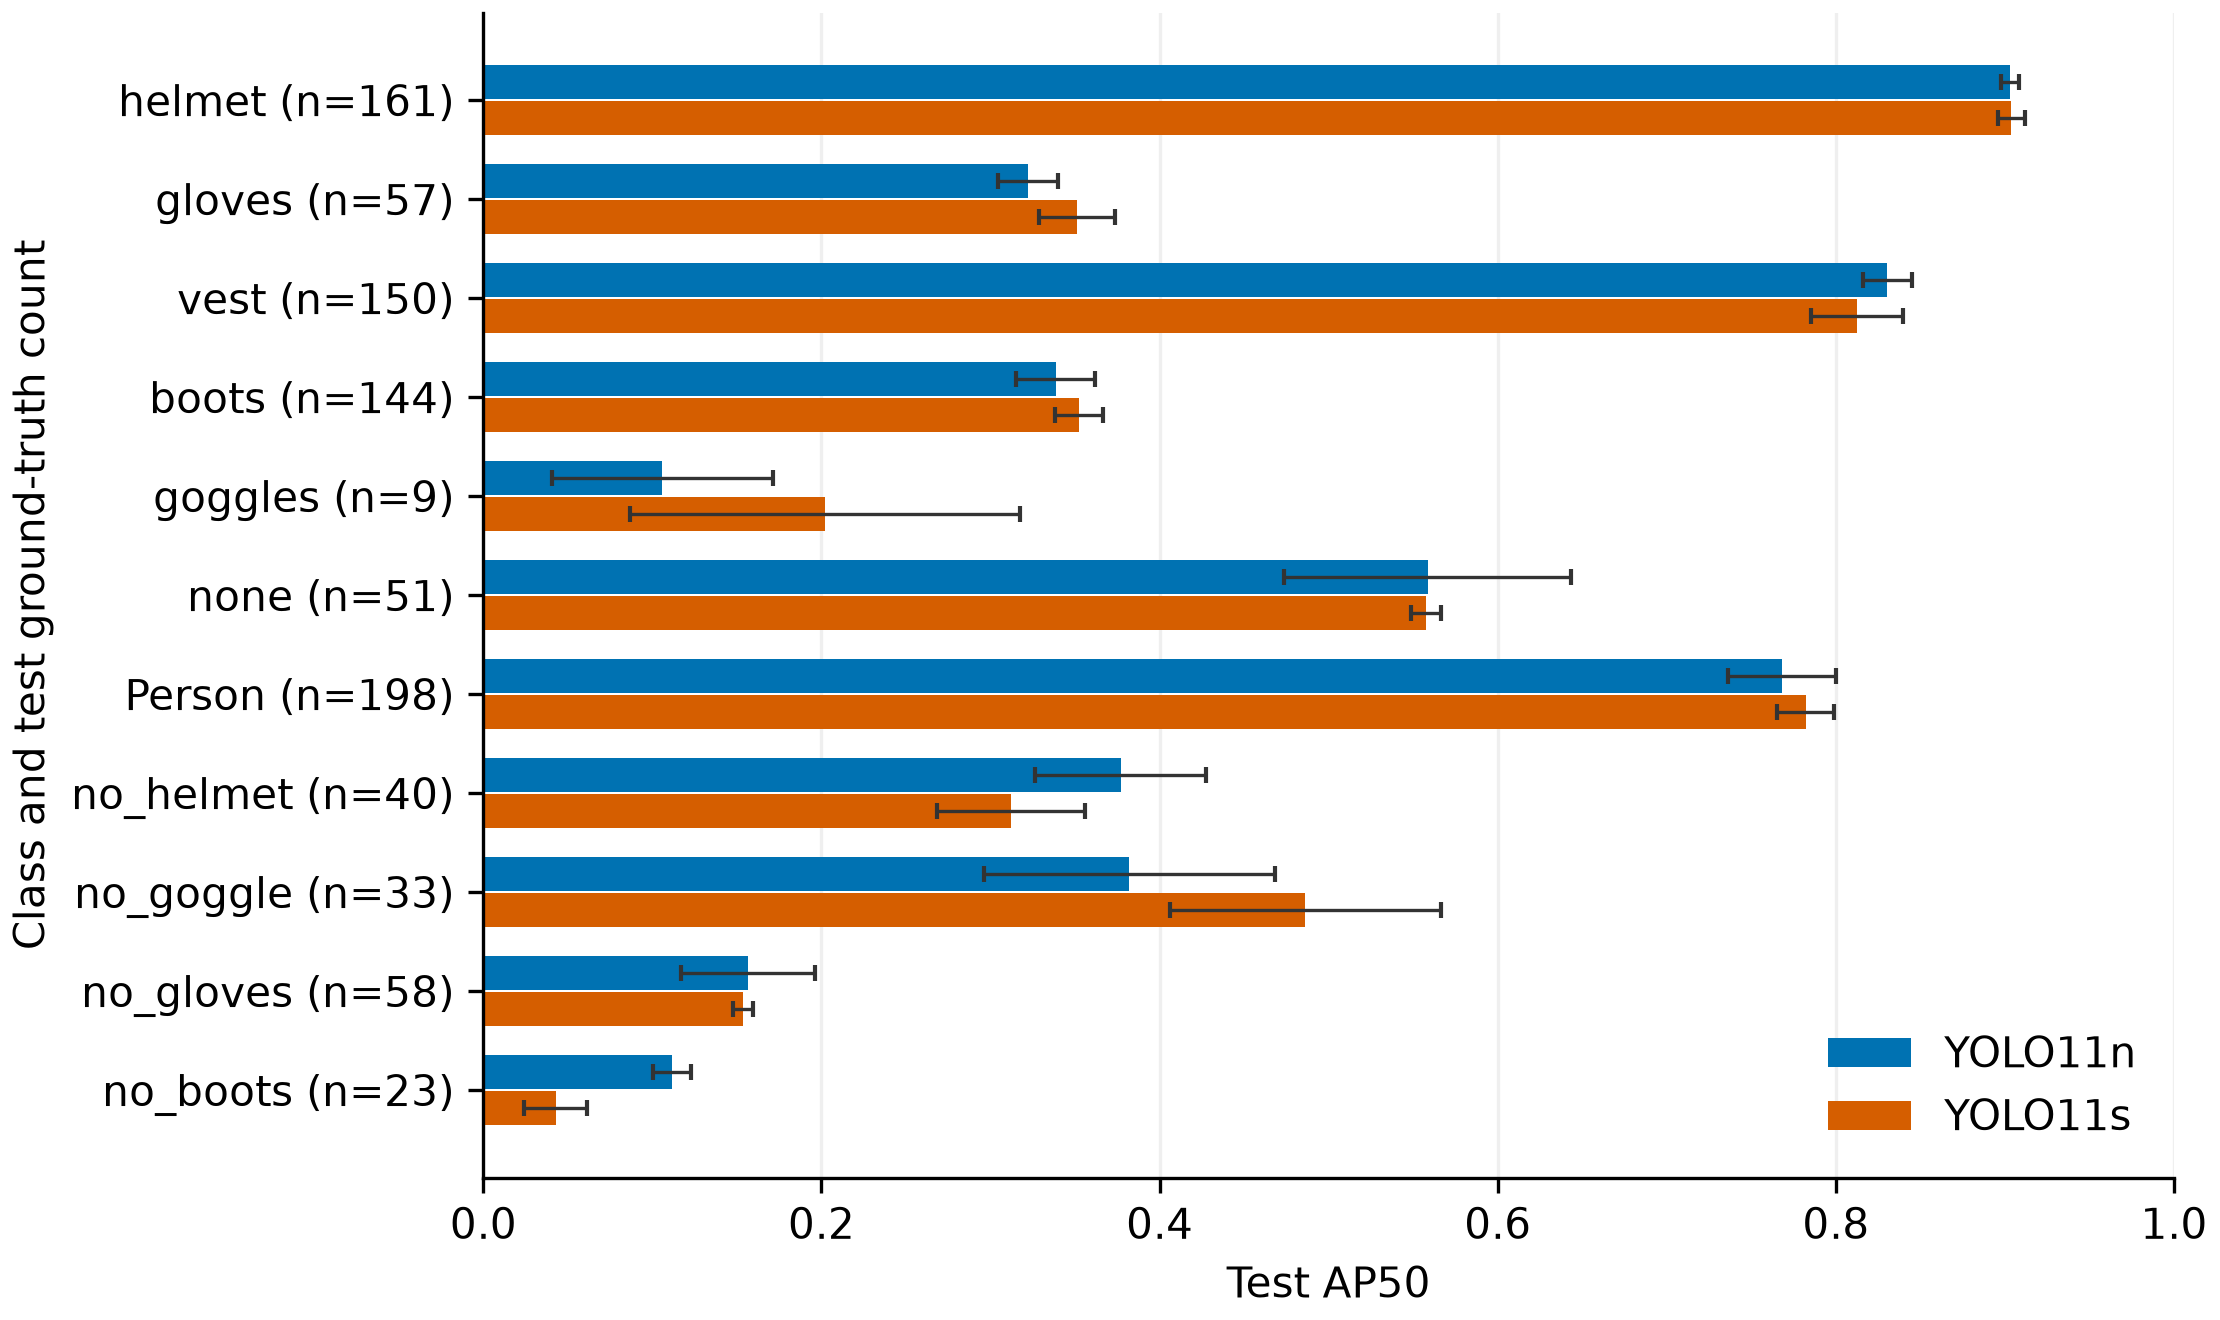
\includegraphics[width=.98\linewidth]{class_ap50_comparison.png}
\end{center}
\textbf{Figure 1. Per-class AP50.} The larger model improves some classes, especially \texttt{goggles} and \texttt{no\_goggle}, but loses performance on \texttt{no\_helmet} and \texttt{no\_boots}. The high variability and nine-object support for goggles limit conclusions. AP uses ranked predictions at confidence 0.001, independently of the fixed deployment thresholds.
\begin{center}
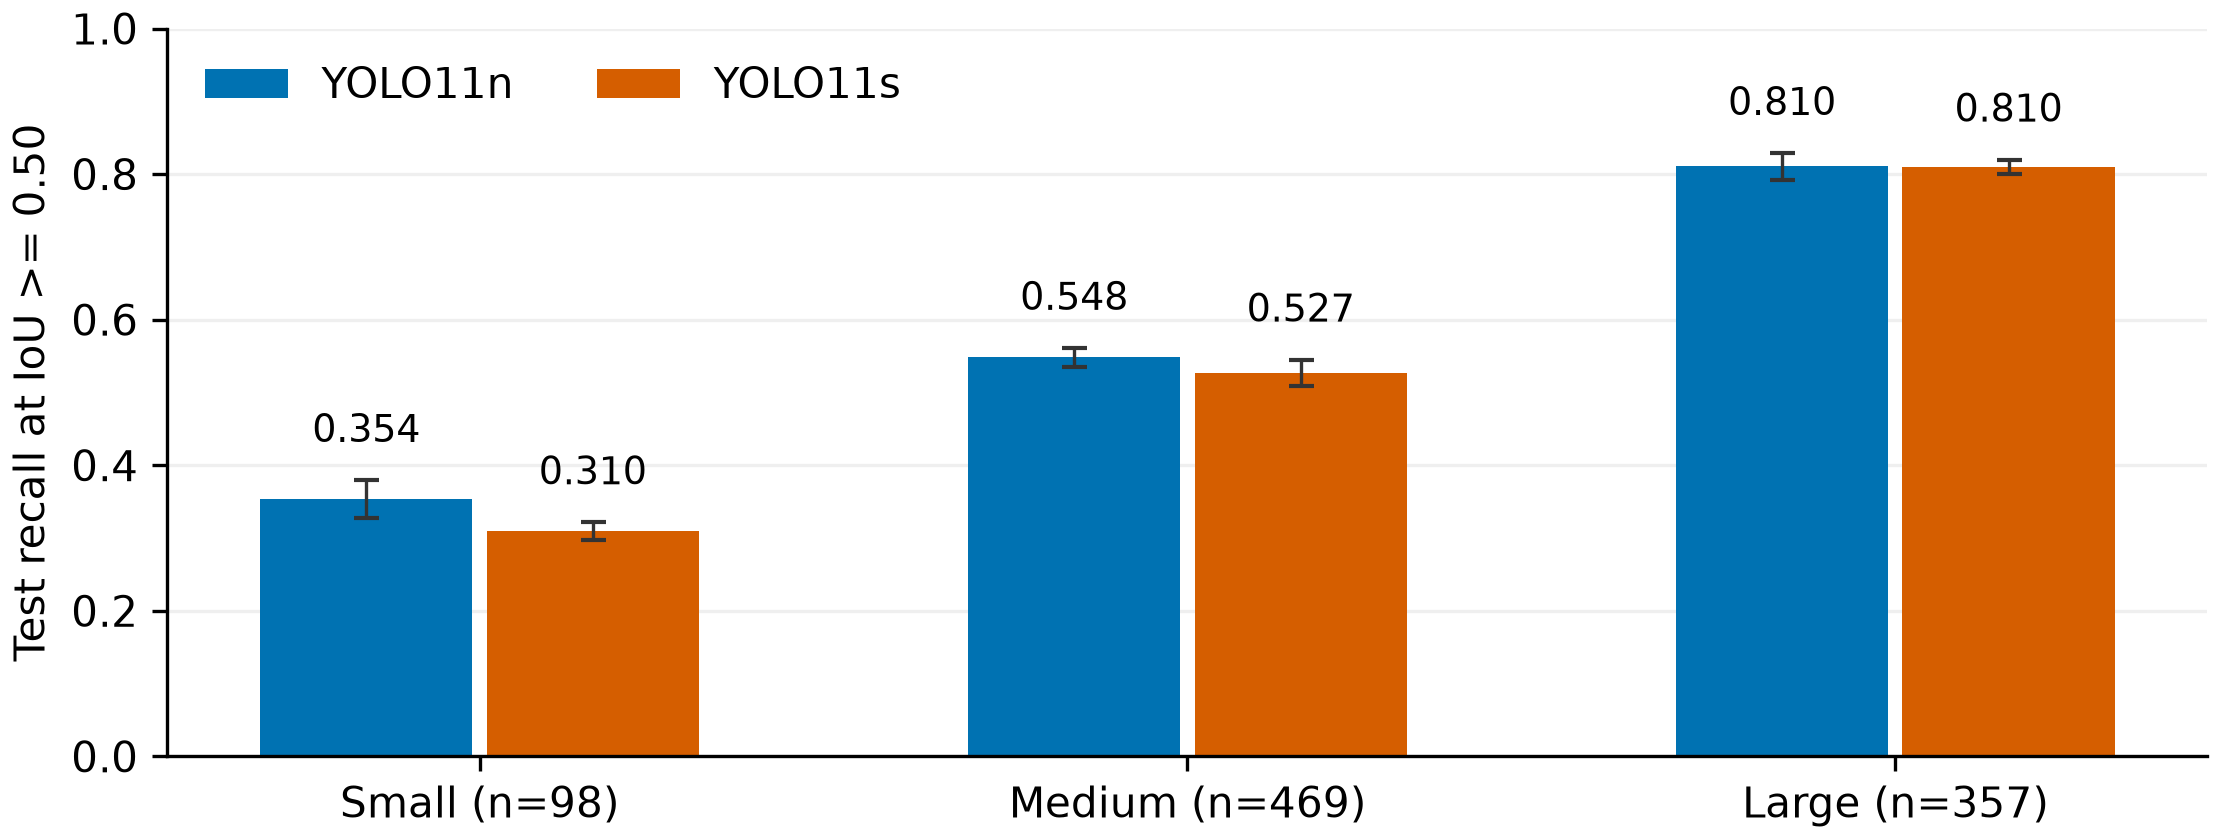
\includegraphics[width=.98\linewidth]{size_recall_comparison.png}
\end{center}
\textbf{Figure 2. Recall by object size.} Small objects have the lowest recall for both models. Recall uses IoU $\geq0.50$ and the frozen confidence thresholds: 0.20 for YOLO11n and 0.30 for YOLO11s. The comparison therefore includes both model and operating-point effects; counts and class composition differ across sizes. All 924 test objects are included, with size boundaries $32^2$ and $96^2$ pixels after resize.
\newpage
\section*{4. Three representative observed failures}
Both columns use seed 42 and the frozen model thresholds. \textbf{Yellow} marks the selected ground-truth object; \textbf{cyan} marks the retained same-class prediction with the highest IoU to that object, when overlap is nonzero. Crops are enlarged for readability; inference used the full image. Examples are illustrative, not estimates of error frequencies. Source image names and original one-based label lines below permit exact recovery.
\begin{center}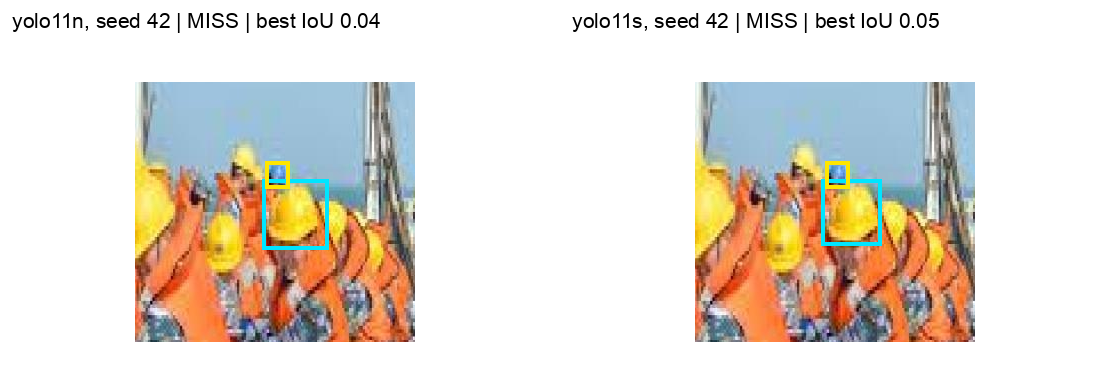
\includegraphics[width=.78\linewidth]{small_miss.png}\end{center}
\textbf{Small-object miss --- \path|images/test/image182.jpg|, line 7, helmet.}
The target occupies approximately $24\times28$ pixels at 640 resolution ($A=661$ px$^2$). Neither model matches it. The cyan boxes belong to a larger neighbouring helmet and are already matched to another target (IoU to this target 0.045/0.050). Limited pixel detail and a crowded, visibly transformed image plausibly explain the miss. Its visibility tag is uncertain; this example is not evidence for an occlusion effect.
\begin{center}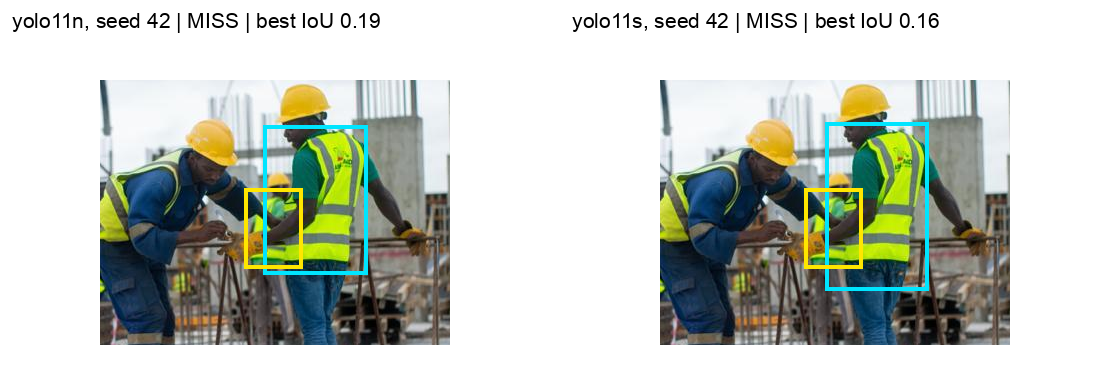
\includegraphics[width=.78\linewidth]{occluded_miss.png}\end{center}
\textbf{Occlusion-associated miss --- \path|images/test/image1037.jpeg|, line 10, vest.}
This medium target has $A=4,671$ px$^2$ and is tagged occluded. The yellow region is partly hidden among overlapping workers and arms. Both models detect the neighbouring worker's larger vest (cyan), already assigned to another target, but not this box (best IoU 0.185/0.159). Occlusion and difficult instance separation are plausible causes. The source vest boundary is also ambiguous, so annotation quality may contribute; this single case does not establish causality.
\begin{center}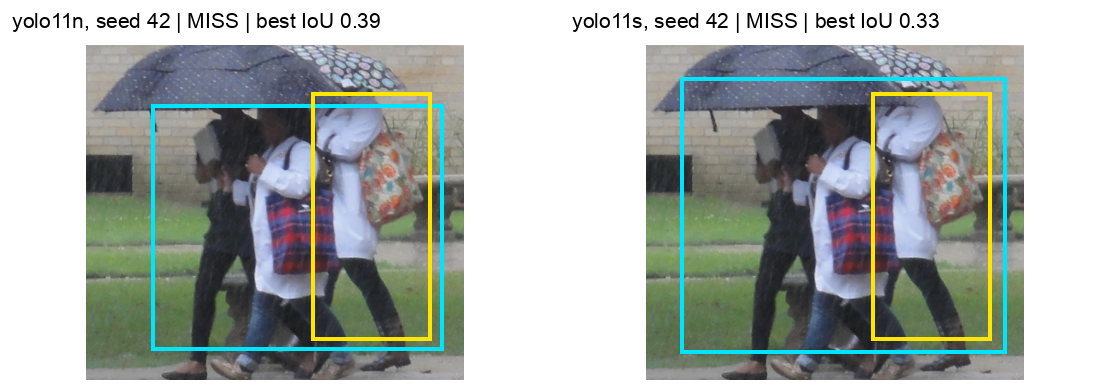
\includegraphics[width=.78\linewidth]{localization.png}\end{center}
\textbf{Localization false positive --- \path|images/test/image1125.jpg|, line 10, Person.}
Both models emit a broad Person box spanning multiple overlapping people under umbrellas. Confidence is 0.837/0.798, yet IoU to the selected person is only 0.387/0.330. Each cyan prediction is unmatched to \emph{any} target at IoU 0.50, making it a false positive; the selected person is also a false negative. Overlap, low contrast and merged silhouettes plausibly cause the localization error. Raising confidence alone would retain these high-confidence errors.
\newpage
\section*{5. Class breakdown of size-dependent recall}
\begin{center}\small\begin{tabular}{lrrrr}
\toprule
Class & Size & Count & Recall (n) & Recall (s) \\
\midrule
helmet & small & 33 & 0.758 $\pm$ 0.030 & 0.727 $\pm$ 0.052 \\
helmet & medium & 111 & 0.907 $\pm$ 0.005 & 0.907 $\pm$ 0.014 \\
helmet & large & 17 & 0.961 $\pm$ 0.068 & 0.980 $\pm$ 0.034 \\
gloves & small & 14 & 0.167 $\pm$ 0.041 & 0.095 $\pm$ 0.041 \\
gloves & medium & 41 & 0.439 $\pm$ 0.049 & 0.415 $\pm$ 0.042 \\
gloves & large & 2 & 0.000 $\pm$ 0.000 & 0.000 $\pm$ 0.000 \\
vest & medium & 54 & 0.809 $\pm$ 0.028 & 0.741 $\pm$ 0.085 \\
vest & large & 96 & 0.847 $\pm$ 0.022 & 0.854 $\pm$ 0.018 \\
boots & small & 16 & 0.354 $\pm$ 0.253 & 0.188 $\pm$ 0.125 \\
boots & medium & 128 & 0.419 $\pm$ 0.063 & 0.401 $\pm$ 0.009 \\
goggles & medium & 9 & 0.037 $\pm$ 0.064 & 0.111 $\pm$ 0.111 \\
none & small & 3 & 0.000 $\pm$ 0.000 & 0.000 $\pm$ 0.000 \\
none & medium & 11 & 0.515 $\pm$ 0.139 & 0.424 $\pm$ 0.052 \\
none & large & 37 & 0.775 $\pm$ 0.041 & 0.766 $\pm$ 0.016 \\
Person & small & 3 & 0.000 $\pm$ 0.000 & 0.000 $\pm$ 0.000 \\
Person & medium & 3 & 0.444 $\pm$ 0.192 & 0.333 $\pm$ 0.000 \\
Person & large & 192 & 0.807 $\pm$ 0.024 & 0.802 $\pm$ 0.014 \\
no\_helmet & small & 3 & 0.000 $\pm$ 0.000 & 0.000 $\pm$ 0.000 \\
no\_helmet & medium & 26 & 0.385 $\pm$ 0.133 & 0.308 $\pm$ 0.067 \\
no\_helmet & large & 11 & 0.697 $\pm$ 0.052 & 0.636 $\pm$ 0.091 \\
no\_goggle & small & 4 & 0.333 $\pm$ 0.144 & 0.417 $\pm$ 0.144 \\
no\_goggle & medium & 29 & 0.437 $\pm$ 0.072 & 0.471 $\pm$ 0.080 \\
no\_gloves & small & 12 & 0.028 $\pm$ 0.048 & 0.028 $\pm$ 0.048 \\
no\_gloves & medium & 44 & 0.212 $\pm$ 0.026 & 0.205 $\pm$ 0.023 \\
no\_gloves & large & 2 & 0.167 $\pm$ 0.289 & 0.500 $\pm$ 0.000 \\
no\_boots & small & 10 & 0.000 $\pm$ 0.000 & 0.000 $\pm$ 0.000 \\
no\_boots & medium & 13 & 0.128 $\pm$ 0.118 & 0.051 $\pm$ 0.044 \\
\bottomrule
\end{tabular}
\end{center}
Support is the number of test boxes in each class/size cell; recall is mean $\pm$ SD over the three seeds. Only nonempty cells are shown. Aggregate size recall must be read together with these counts. Goggles and several missing-equipment cells have very limited support.
\section*{6. Interpretation and reproducibility}
YOLO11s improves mean test macro-F1, but provides only a small AP gain, costs about 3.6 times as many parameters and \LatencyRatio{} times the CPU latency, and does not solve small-object or missing-equipment failures. YOLO11n remains a reasonable efficiency baseline; YOLO11s is preferable when the measured precision/F1 gain matters more than latency. These observations apply to this fixed test set and operating points. Three seeds measure training variability on one split; they do not measure uncertainty over new sites. Dataset labels identify equipment categories without assigning PPE to individual workers.

The report uses the retained reproduction checkpoints. The lost Stage 3 T4 experiment is historical and is not included in test aggregates. The test split was used only after Stage 4 selection; future changes should be tuned on validation or new development data. No additional training was needed for this checkpoint.

\textbf{Reproduce from the repository root:}
\begin{verbatim}
.venv/bin/python scripts/evaluate_test.py --device cpu --benchmark
.venv/bin/python scripts/build_results_report.py
\end{verbatim}
In \texttt{planning/latex}, compile \texttt{results\_checkpoint.tex} with Tectonic or run pdfLaTeX twice. Preparation and output details are documented in the Results checkpoint README. Checkpoint, test-content, annotation and validation-summary SHA-256 values are retained in JSON provenance records. Caches require matching content and environment fingerprints.

{\raggedright\textbf{Evidence:} the test summary, per-seed/per-class/subgroup CSVs and \texttt{failure\_examples.json} in \texttt{reports/results\_checkpoint}; Stage 4 validation summary; retained training logs; dataset split manifest and visibility review. Source attribution and archive checksum are in \texttt{data/ATTRIBUTION.md} and \texttt{data/source.json}. Repository: \url{https://github.com/Ta6leTkaa/intro-to-CV-Project}.\par}
\end{document}
